
%%%%%%%%%%%%%%%%%%%%%%%%%%%%%%%%%%%%%%%%%%%%%%%%%%%%%%%%%%%%%%%%%%%%%%%%%%%%%
%% Descr:       Vorlage für Berichte der DHBW-Karlsruhe, Ein Kapitel
%% Author:      Prof. Dr. Jürgen Vollmer, vollmer@dhbw-karlsruhe.de
%% $Id: kapitel2.tex,v 1.5 2017/10/06 14:02:51 vollmer Exp $
%%  -*- coding: utf-8 -*-
%%%%%%%%%%%%%%%%%%%%%%%%%%%%%%%%%%%%%%%%%%%%%%%%%%%%%%%%%%%%%%%%%%%%%%%%%%%%%%%

\chapter{Umsetzung}
\label{chap:Umsetzung}
Dieses Kapitel greift die in der Konzeption (\ref{chap:Konzeption}) aufgeführten Planungen und Ideen auf und geht auf Details bei der 
Implementierung ein. Darunter Lösungsansätze, aufgetretene Probleme und deren Behebung. Allgemein die Umsetzung der beiden Kernfunktionen 
sowohl die FrontEnd als auch die BackEnd Aspekte werden in der Implementierung (\ref{chap:implementierung}) aufgezeigt. Abschließend zu 
dem Kapitel wird ein Szenario dargestellt, indem die Anwendung beschrieben wird.

\section{Implementierung}
\label{chap:implementierung}

\subsection{Startmenü}
\subsubsection{FrontEnd}
\begin{figure}[hbt!]
    \centering
    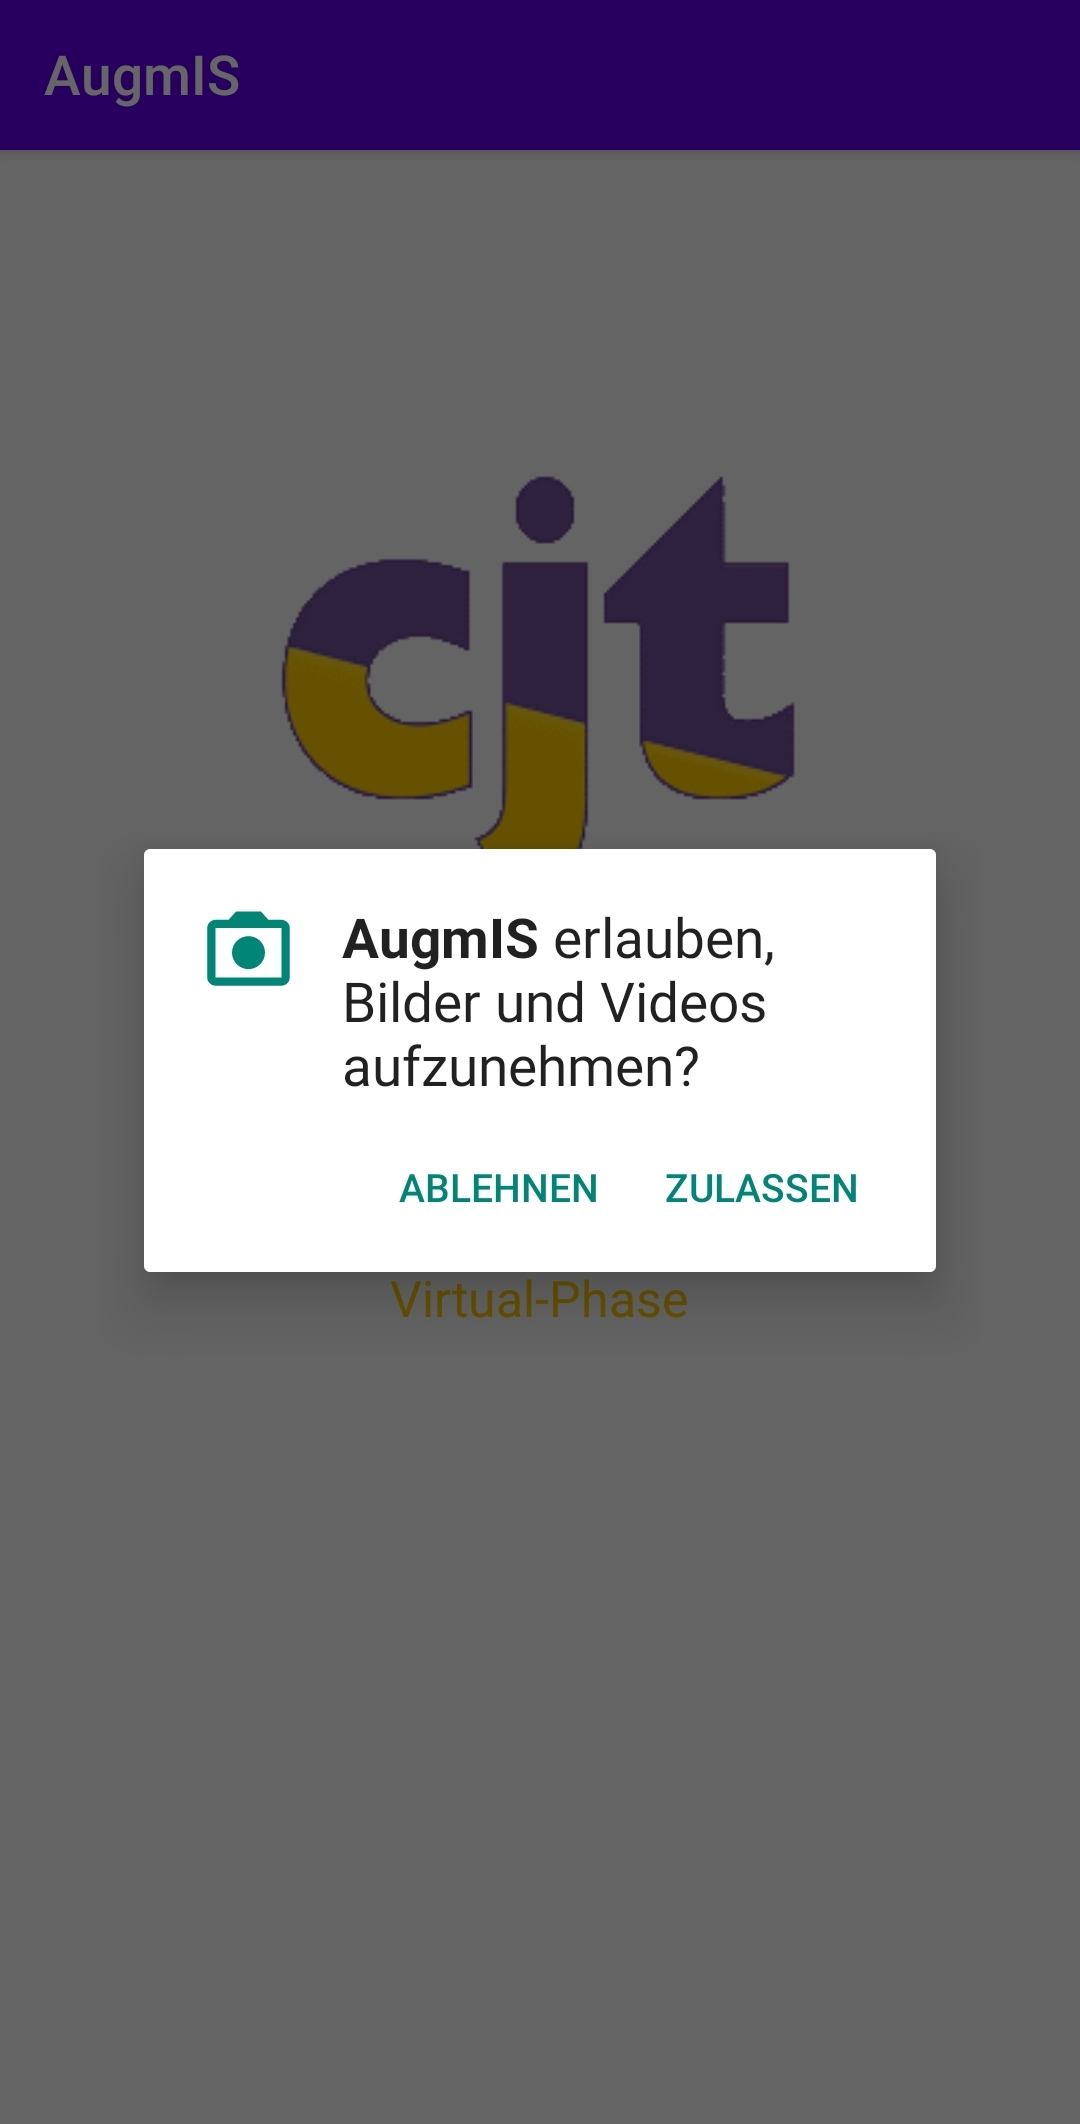
\includegraphics[width=10cm,height=7.5cm,keepaspectratio]{4Umsetzung/Bilder/camera_permission.jpg}
    \caption{Start der Applikation}
    \label{pic:camera_perm}
\end{figure}
\begin{figure}[hbt!]
    \centering
    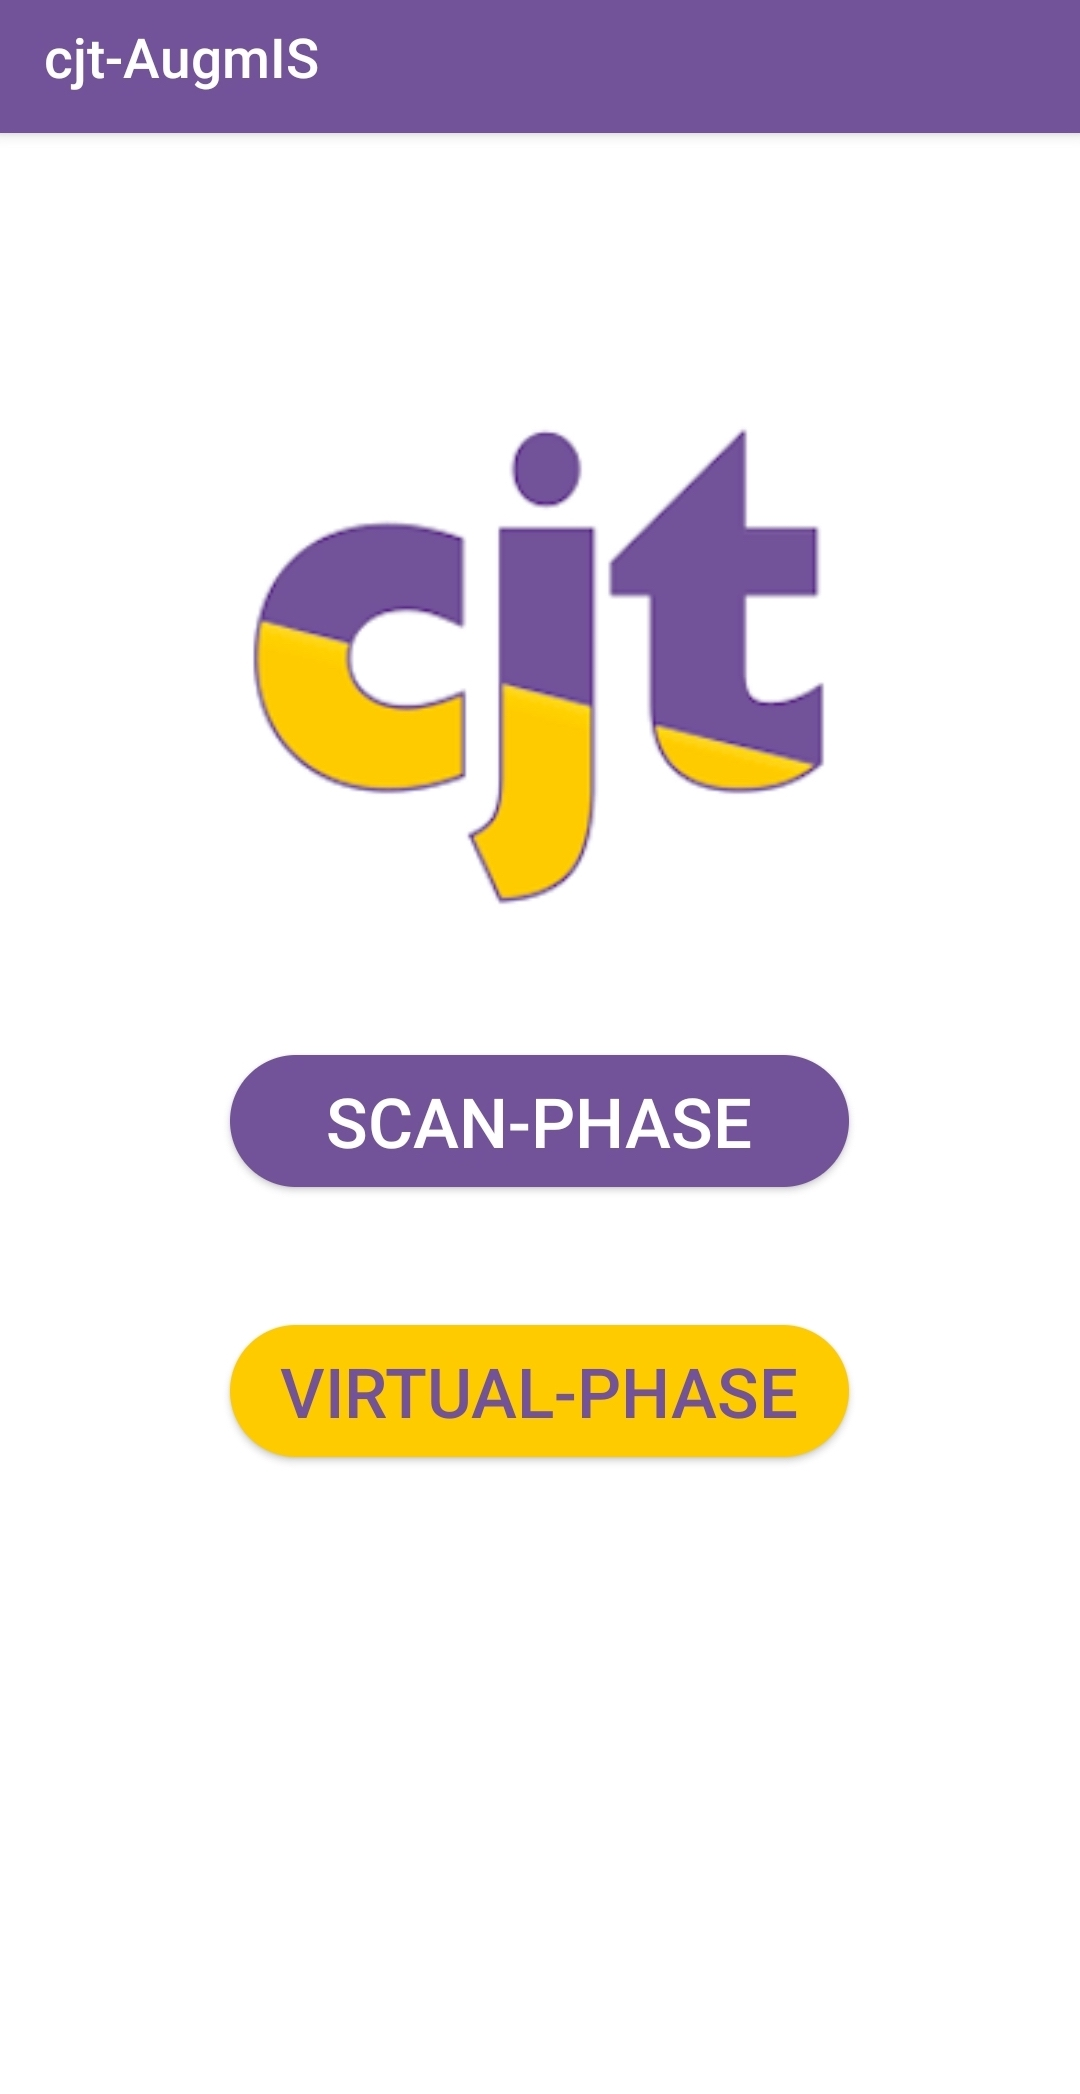
\includegraphics[width=10cm,height=7.5cm,keepaspectratio]{4Umsetzung/Bilder/startmenu.jpg}
    \caption{Startmenü der Applikation}
    \label{pic:startmenu}
\end{figure}
\subsubsection{BackEnd}

\subsection{Scan-Phase} %Umgebungserkennung /
\subsubsection{FrontEnd}
\begin{figure}[hbt!]
    \centering
    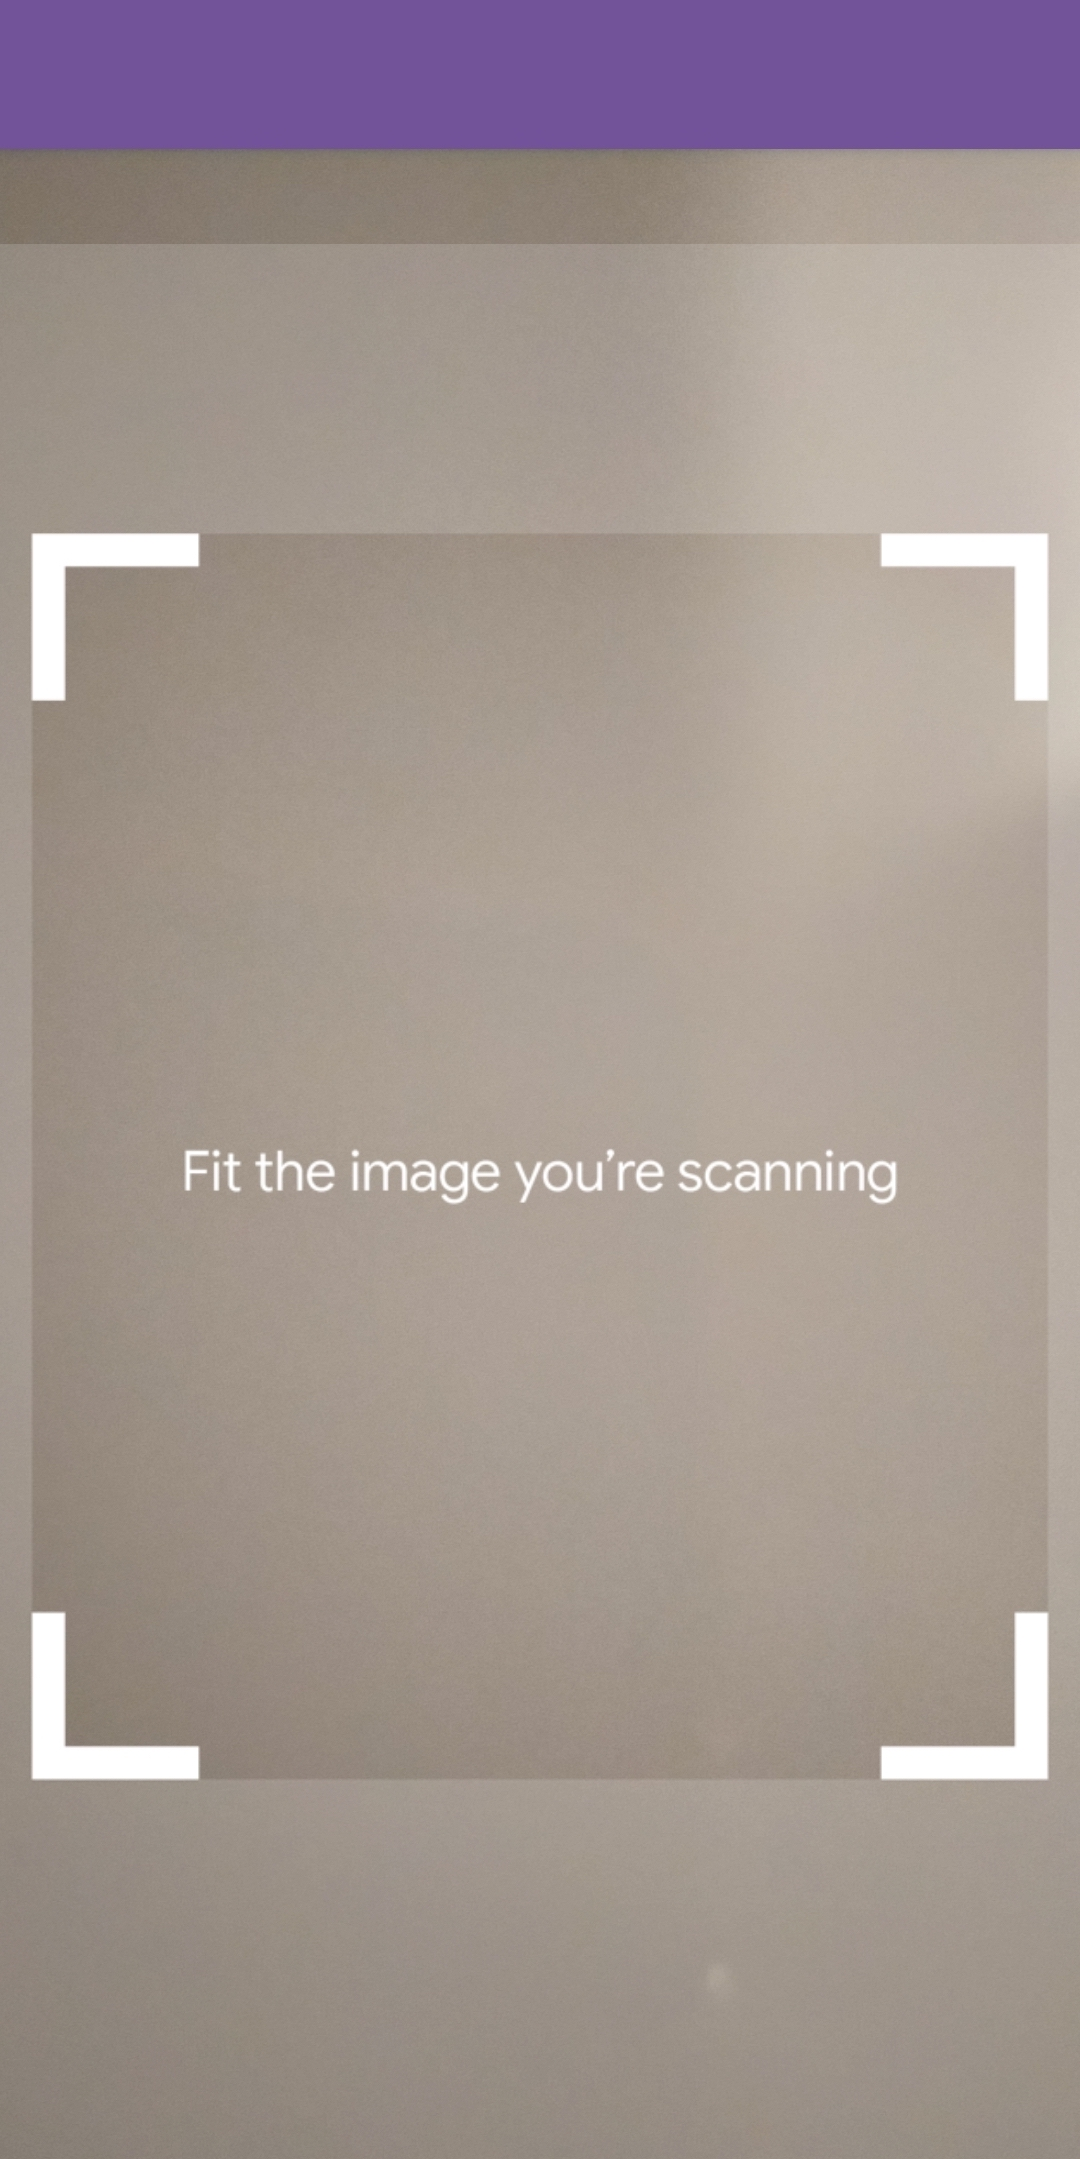
\includegraphics[width=10cm,height=7.5cm,keepaspectratio]{4Umsetzung/Bilder/image_tracking.jpg}
    \caption{Markererkennung der Applikation zum Start der Scan-Phase}
    \label{pic:image_tracking}
\end{figure}
\begin{figure}[hbt!]
    \centering
    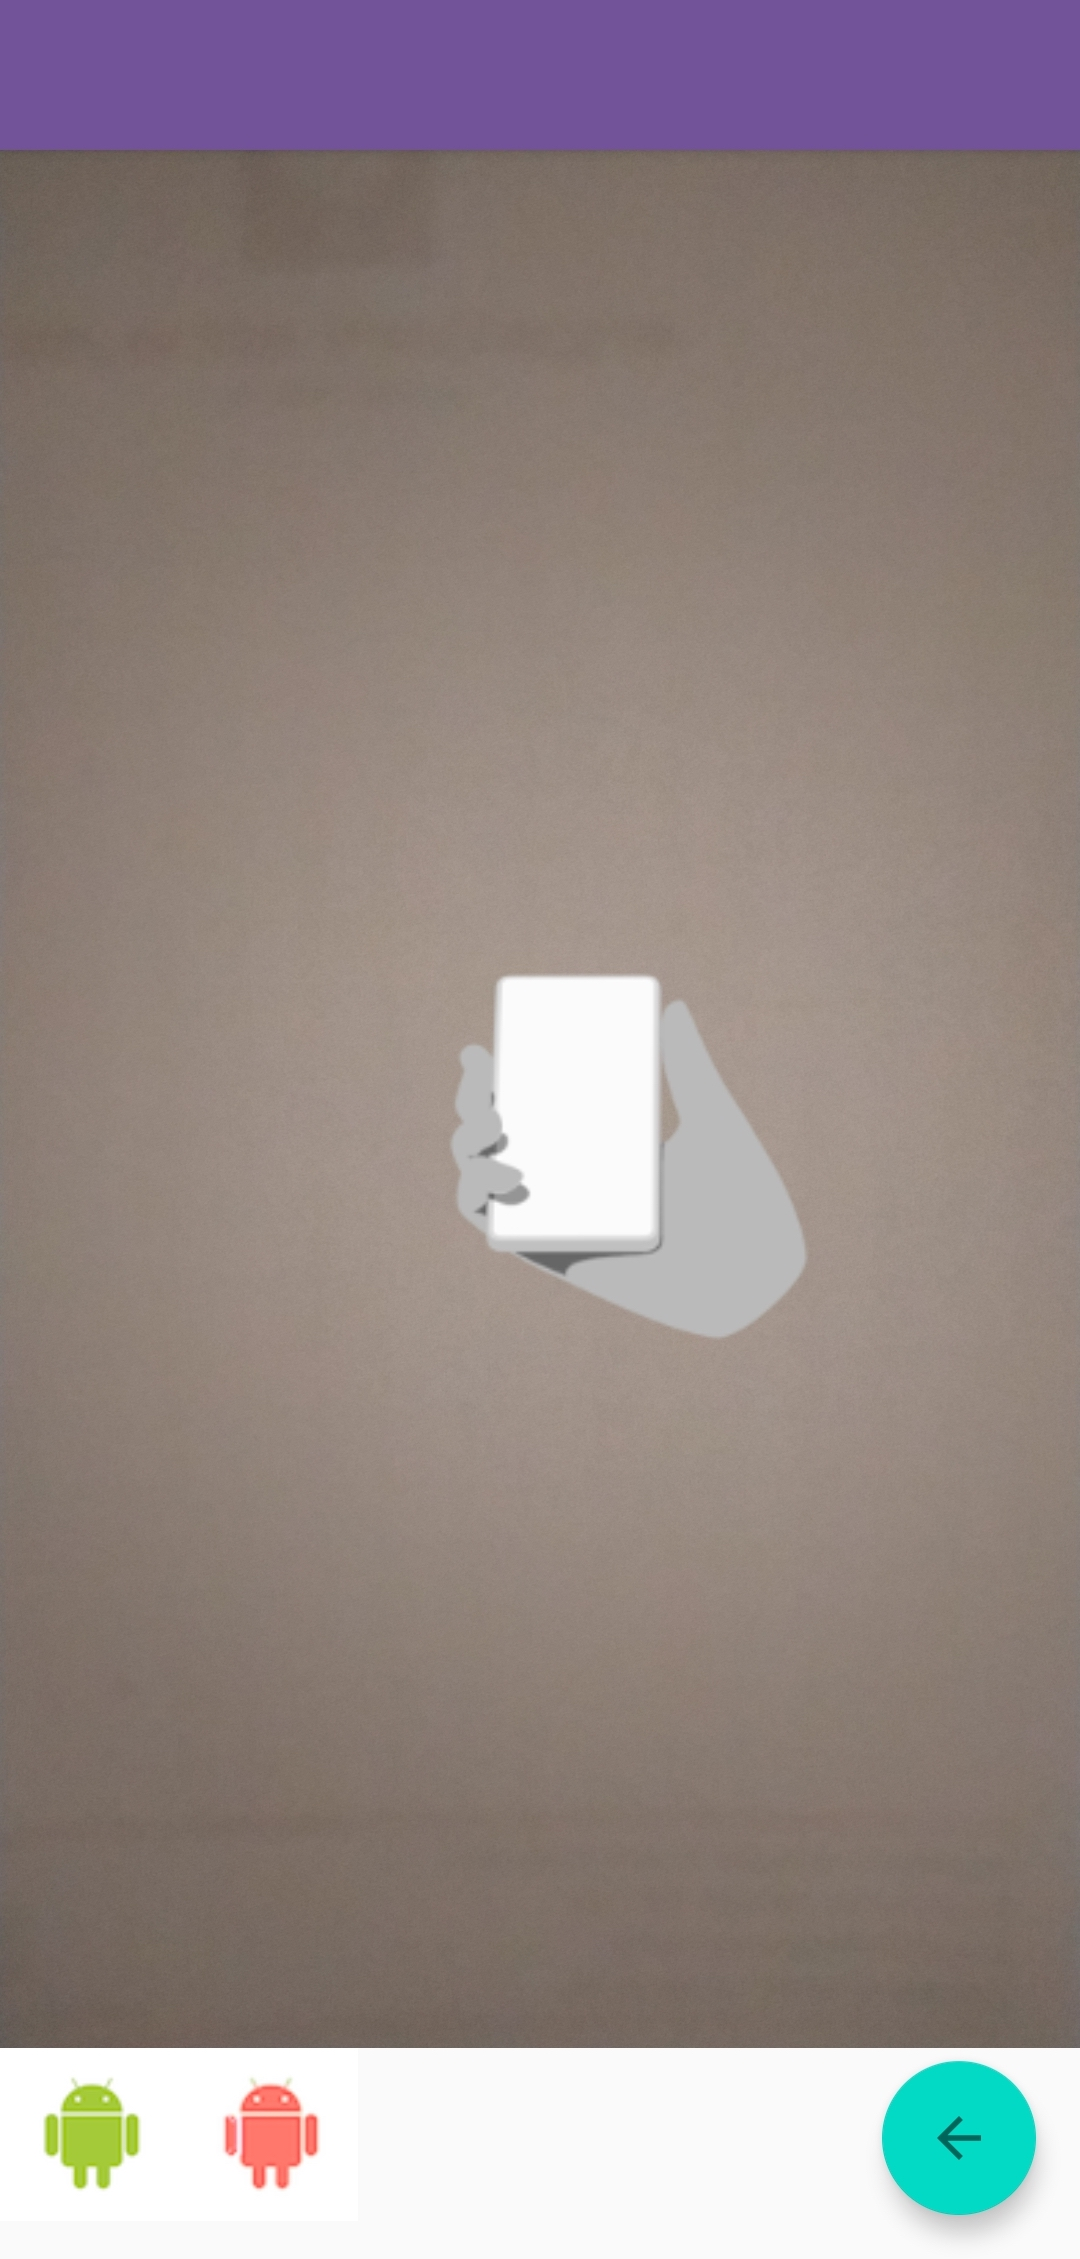
\includegraphics[width=10cm,height=7.5cm,keepaspectratio]{4Umsetzung/Bilder/scan-phase.jpg}
    \caption{Scan-Phase der Applikation}
    \label{pic:scan}
\end{figure}
\subsubsection{BackEnd}
\begin{figure}[hbt!]
    \centering
    
\includegraphics[width=5cm,height=5cm,keepaspectratio]{4Umsetzung/Bilder/cjt_logo_tracking.png}
    \caption{Marker zur Erkennung der Ausgangsposition}
    \label{pic:initialMarker}
\end{figure}

\subsection{Visualisierungs-Phase} 
\subsubsection{FrontEnd}
\begin{figure}[hbt!]
    \centering
    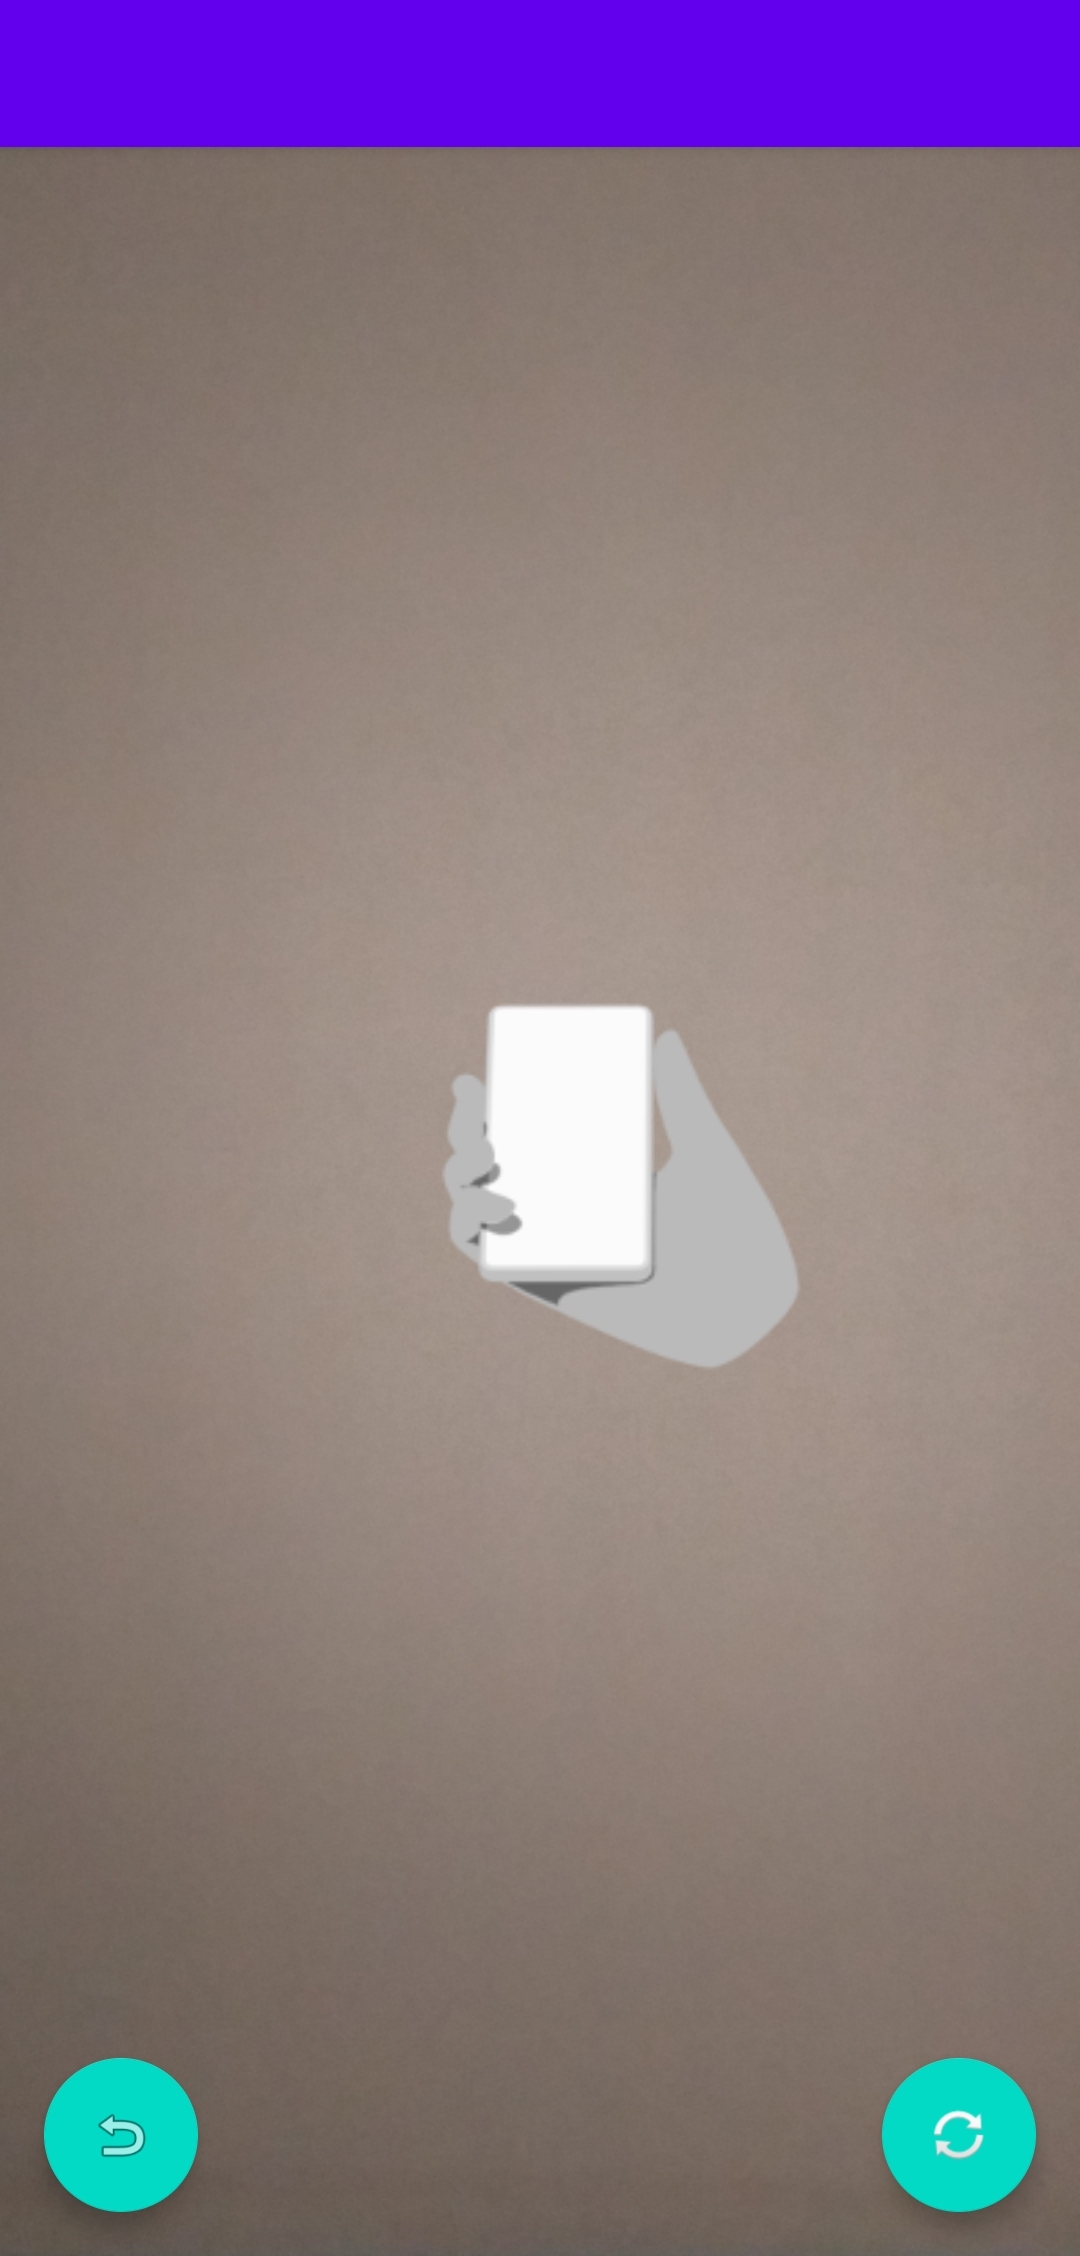
\includegraphics[width=10cm,height=7.5cm,keepaspectratio]{4Umsetzung/Bilder/visual-phase.jpg}
    \caption{Visualisierungs-Phase der Applikation}
    \label{pic:visual}
\end{figure}
\subsubsection{BackEnd}

\section{Testdurchlauf / Test-Szenario}
\label{chap:testdurchlauf}